
%(BEGIN_QUESTION)
% Copyright 2010, Tony R. Kuphaldt, released under the Creative Commons Attribution License (v 1.0)
% This means you may do almost anything with this work of mine, so long as you give me proper credit

The amount of pressure inside this high-pressure chemical reactor vessel is controlled by a pressure control valve (PCV) at top, and is measured by a ``DP'' style of pressure transmitter connected to the reactor through a ``block-and-bleed'' valve manifold:

$$\includegraphics[width=15.5cm]{i04576x01.eps}$$

Suppose an instrument technician is told to remove the pressure transmitter from service in order to check its calibration.  Explain what will happen (and why!) if a technician happens to close the transmitter's block valve and open the bleed valve while the pressure controller (PIC) is in automatic mode.

\vskip 20pt \vbox{\hrule \hbox{\strut \vrule{} {\bf Suggestions for Socratic discussion} \vrule} \hrule}

\begin{itemize}
\item{} Describe a better way of removing the transmitter from service!
\item{} If this pressure control loop were implemented on FOUNDATION Fieldbus, would it be best to have a minimum number of devices on the H1 segment?  Why or why not?
\end{itemize}

\underbar{file i04576}
%(END_QUESTION)





%(BEGIN_ANSWER)

The device labeled ``PRV'' will begin to make a very loud noise . . . and the technician might die.  And you thought this was going to be a boring, academic exercise?!

\vskip 10pt

Seriously, be prepared to explain exactly {\it why} these very bad things might happen in this system.

%(END_ANSWER)





%(BEGIN_NOTES)


%INDEX% Basics, control loop troubleshooting: determining effect of specified fault(s)
%INDEX% Process: reactor pressure control (generic)

%(END_NOTES)

